\documentclass[tikz,border=5mm,12pt]{standalone}
\usetikzlibrary{backgrounds}

\newcommand\edge{12mm}

\begin{document}
  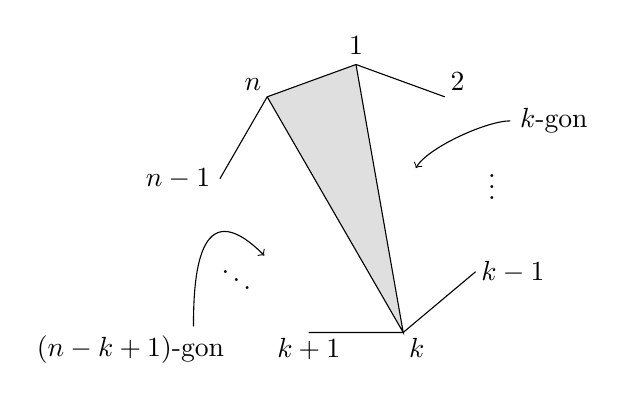
\begin{tikzpicture}
    \path (0,0) coordinate (P1)
      -- ++(340:\edge) coordinate (P2)
      -- ++(300:\edge) coordinate (P3)
      -- ++(260:\edge) coordinate (P4)
      -- ++(220:\edge) coordinate (P5)
      -- ++(180:\edge) coordinate (P6)
      -- ++(140:\edge) coordinate (P7)
      -- ++(100:\edge) coordinate (P8)
      -- ++(60:\edge) coordinate (P9)
      -- cycle;

    % partially draw edges
    \draw (P8) -- (P9) -- (P1) -- (P2);
    \draw (P4) -- (P5) -- (P6);

    % label
    \node[above]              at (P1) {1};
    \node[above right=-0.5mm] at (P2) {2};
    \node                     at (P3) {$\vdots$};
    \node[right=-0.5mm]       at (P4) {$k-1$};
    \node[below right=-0.5mm] at (P5) {$k$};
    \node[below=-0.5mm]       at (P6) {$k+1$};
    \node                     at (P7) {$\ddots$};
    \node[above left=-0.5mm]  at (P9) {$n$};
    \node[left]               at (P8) {$n-1$};

    % shaded triangle
    \draw (P1) -- (P5) -- (P9);
    \begin{scope}[on background layer]
      \fill[lightgray!50] (P1) -- (P5) -- (P9) -- cycle;
    \end{scope}

    % right annotation
    \path (P1) -- (P4) coordinate[midway] (P14);
    \draw[<-] (P14) .. controls +(60:3mm) and +(left:3mm) .. ++(12mm,6mm) coordinate (R);
    \node[right] at (R) {$k$-gon};

    % left annotation
    \path (P6) -- (P8) coordinate[midway] (P68);
    \draw[<-] (P68) .. controls +(135:12mm) and +(90:6mm) .. ++(-9mm,-9mm) coordinate (L);
    \node[below=0mm,xshift=-8mm] at (L) {$(n-k+1)$-gon};
  \end{tikzpicture}
\end{document}
